% This is main.tex, demonstrating the LLNCS macro package for Springer Computer Science proceedings;
% Version 2.21 of 2022/01/12
%
\documentclass[runningheads]{llncs}
%
\usepackage[T1]{fontenc}
% T1 fonts will be used to generate the final print and online PDFs,
% so please use T1 fonts in your manuscript whenever possible.
% Other font encondings may result in incorrect characters.
%
\usepackage{graphicx}
% Used for displaying a sample figure. If possible, figure files should
% be included in EPS format.
%
% Include custom macros and mathematical packages
% ==============================================================================
% Mathematical Notation and Custom Macros for OrthoStyle Paper
% ==============================================================================

% Springer LNCS and amsmath compatibility for \vec
\let\accentvec\vec
\usepackage{amsmath,amssymb,amsfonts}
\let\spvec\vec
\let\vec\accentvec
\usepackage{bm}
\usepackage{xspace}
\usepackage{booktabs}
\usepackage{multirow}
\usepackage{graphicx}
\usepackage{hyperref}
\usepackage{url}
\usepackage{xcolor}
\usepackage{algorithm}
\usepackage{algorithmic}

% Method Name
\newcommand{\method}{\textsc{OrthoStyle}\xspace}
\newcommand{\ours}{\textsc{OrthoStyle}\xspace}

% Math Vectors and Matrices
\newcommand{\bx}{\mathbf{x}}
\newcommand{\bz}{\mathbf{z}}
\newcommand{\by}{\mathbf{y}}
\newcommand{\bc}{\mathbf{c}}
\newcommand{\bs}{\mathbf{s}}
\newcommand{\bg}{\mathbf{g}}
\newcommand{\bv}{\mathbf{v}}
\newcommand{\bu}{\mathbf{u}}
\newcommand{\bk}{\mathbf{k}}
\newcommand{\bq}{\mathbf{q}}
\newcommand{\beps}{\boldsymbol{\epsilon}}
\newcommand{\btheta}{\boldsymbol{\theta}}
\newcommand{\bmu}{\boldsymbol{\mu}}
\newcommand{\bsigma}{\boldsymbol{\sigma}}

% Subspaces and Operators
\newcommand{\Vsub}{\mathcal{V}_{\text{sub}}}
\newcommand{\Vortho}{\mathcal{V}_{\text{sub}}^\perp}
\newcommand{\Proj}{\text{Proj}}
\newcommand{\norm}[1]{\left\lVert#1\right\rVert}
\newcommand{\inner}[2]{\left\langle #1, #2 \right\rangle}
\newcommand{\E}{\mathbb{E}}
\newcommand{\R}{\mathbb{R}}
\newcommand{\Loss}{\mathcal{L}}

% Attention Variables
\newcommand{\xtxt}{\mathbf{x}_{\text{txt}}}
\newcommand{\xsub}{\mathbf{x}_{\text{sub}}}
\newcommand{\xstyle}{\mathbf{x}_{\text{style}}}
\newcommand{\xsubstyle}{\mathbf{x}_{\text{sub\_style}}}
\newcommand{\xstyleortho}{\mathbf{x}_{\text{style}}^\perp}
\newcommand{\xsubstyleortho}{\mathbf{x}_{\text{sub\_style}}^\perp}
\newcommand{\wtxt}{w_{\text{txt}}}
\newcommand{\wsub}{w_{\text{sub}}}
\newcommand{\wstyle}{w_{\text{style}}}
\newcommand{\wsubstyle}{w_{\text{sub\_style}}}

% Formatting helpers
\newcommand{\best}[1]{\textbf{#1}}
\newcommand{\second}[1]{\underline{#1}}
\newcommand{\fixme}[1]{\textcolor{red}{[FIXME: #1]}}
\newcommand{\todo}[1]{\textcolor{blue}{[TODO: #1]}}


\begin{document}
%
\title{\method: Manifold-Preserving Training-Free Style Transfer via Score-Orthogonal Guidance}
%
\titlerunning{\method: Manifold-Preserving Training-Free Style Transfer}
%
\author{Nhat Minh Nguyen\inst{1,2} \and
Quang Dang Pham\inst{1,2}\and
Phuc Thien Vo\inst{1,2}\and
Loc Phuc Dang\inst{1,2}\and
Khoan Duc Le\inst{1,2}\thanks{Corresponding author}}
%
\authorrunning{N.Nhat et al.}
% First names are abbreviated in the running head.
% If there are more than two authors, 'et al.' is used.
%
\institute{Faculty of Information Technology, University of Science, Ho Chi Minh City, Vietnam \\
\email{\{2512021580, 2512022643, 2512022237, 2512020320\}@student.hcmus.edu.vn}\\
\email{ldkhoan@fit.hcmus.edu.vn}
\and
Vietnam National University, Ho Chi Minh City, Vietnam
}
%
\maketitle
%
\begin{abstract}
Reference-based style transfer with diffusion models aims to synthesize artistic textures while preserving the geometry and semantics of a target image. However, training-free methods face a trade-off between style fidelity and content preservation: strong style injection can distort structure and cause content leakage, while conservative transfer often leads to under-stylization. We introduce \method, a training-free framework that addresses this trade-off without network fine-tuning or DDIM inversion. \method consists of three components: Semantic Gating to preserve structural and semantic cues; Score-Orthogonal DINO Guidance to project style gradients orthogonally to the diffusion score direction, preserving the sampling trajectory near the data manifold; and an Early Step Controller that applies AdaIN-based clean-latent pushforward to establish color and layout before fine-grained stylization. Extensive quantitative and qualitative comparisons with both OC-based baselines and representative stylization methods show that \method achieves a favorable balance between style fidelity and content preservation while maintaining structural consistency. Most notably, it completely outperforms the baseline that uses the same Stable Cascade backbone.

\keywords{Style Transfer \and Training-free \and Score-Orthogonal Guidance \and Diffusion Models.}
\end{abstract}

\section{Introduction}
\label{sec:intro}

Text-to-Image (T2I) diffusion models~\cite{sd,wuerstchen,ddpm} have demonstrated extraordinary capabilities in synthesizing visually compelling and photorealistic imagery from natural language descriptions. These foundation models are increasingly harnessed across diverse creative industries, including digital art creation, video game asset design, personalized concept synthesis, and image editing~\cite{prompt2prompt,instructpix2pix}. Content creators and digital artists typically demand granular, independent control over both the semantic content and the visual style of synthesized images to fulfill their creative vision. While the semantic content of a scene (e.g., "a vintage clock on a wooden table" or "a sitting cat") can be precisely articulated via descriptive text prompts, conveying an artist's signature visual style---characterized by intricate brushstroke impasto, delicate pigment dispersion, non-Euclidean geometric tiling, and distinctive physical medium properties (e.g., oil painting, stained glass, woodblock printing, origami, glowing neon cyberpunk)---is inherently non-verbal, abstract, and vastly more complex. Consequently, communicating these subtle stylistic nuances through text prompts alone is severely hindered by prompt ambiguity and lexical constraints. This has established visual style personalization via visual prompting from a single exemplar image as an indispensable frontier in generative computer vision~\cite{stylealigned,instantstyle,rout2025rbmodulation}.

% ==============================================================================
% Teaser Figure: Comprehensive Qualitative Matrix (Content x Style)
% ==============================================================================
\begin{figure*}[t]
\centering
\includegraphics[width=\textwidth]{figs/qualitative_matrix_teaser.png}
\caption{\textbf{Qualitative Stylization Matrix of \method across Diverse Content Categories and Artistic Styles.} 
Rows depict representative content targets spanning diverse semantic domains (animals, household artifacts, and footwear); columns correspond to diverse artistic styles (oil paintings, mosaic tile art, woodblock prints, glowing neon cyberpunk, and 3D renders). All results are synthesized under null-prompt inference (without text prompt conditioning, akin to RB-Modulation~\cite{rout2025rbmodulation}), demonstrating faithful subject geometry retention while authentically rendering rich stroke dynamics and textural nuances without semantic content leakage.}
\label{fig:teaser_matrix}
\end{figure*}

To personalize pre-trained T2I diffusion models for a target artistic style, existing research predominantly follows two overarching paradigms: (1) fine-tuning-based optimization and (2) training-free inference-time modulation. Fine-tuning approaches---exemplified by DreamBooth~\cite{dreambooth}, Custom Diffusion, LoRA~\cite{lora}, ZipLoRA~\cite{ziplora}, StyleDrop~\cite{styledrop}, and B-LoRA~\cite{b-lora}---optimize the model's text embeddings, cross-attention projection matrices, or low-rank residual weights via the denoising diffusion objective. When fine-tuned on a curated set of multiple reference images (typically 4--10 exemplars of the same artistic domain), these methods can effectively capture stylistic patterns. However, they suffer from three fundamental drawbacks:
(i) curating multiple high-quality images sharing an identical artistic style is often impractical or impossible, particularly for unique historical artworks or bespoke digital designs;
(ii) optimizing model weights for every novel style incurs prohibitive computational cost and latency (requiring several minutes of GPU gradient descent per concept); and
(iii) critically, when constrained to a \textit{single reference exemplar}, fine-tuning methods suffer from severe semantic memorization and catastrophic overfitting---the network inadvertently memorizes and reproduces the concrete semantic objects depicted in the reference artwork (e.g., a specific portrait or building) rather than isolating its abstract stylistic essence.

To overcome the heavy computational burden and multi-image dependency of fine-tuning, recent efforts have focused on training-free personalization by directly manipulating keys, values, and feature maps within the attention layers of pre-trained diffusion models at inference time~\cite{stylealigned,instantstyle,styleid,diffstyler,freestyle}. Nevertheless, existing training-free frameworks confront severe challenges in isolating style from semantic content and transferring it faithfully without structural artifacts. For instance, StyleAligned~\cite{stylealigned} and Swapping Self-Attention (SSA) synchronize style across images by sharing self-attention keys and values. However, these methods rely on deterministic DDIM inversion~\cite{DDIM} to cache reference representations, which inherently compromises high-frequency textural details and accumulates discretization errors; furthermore, they require dual coupled reverse diffusion processes that double GPU memory footprint and runtime. To circumvent DDIM inversion, InstantStyle~\cite{instantstyle} injects reference style features into heuristic subsets of cross-attention layers within a pre-trained IP-Adapter~\cite{ipadapter}. However, manually identifying optimal injection layers is brittle, ad-hoc, and fails to generalize across diverse network architectures. More detrimentally, linear feature injection directly induces catastrophic \textbf{content leakage}---inadvertently synthesizing foreign semantic objects from the style reference into the generated scene (e.g., painting extraneous dragons or houses when only a metallic golden texture was desired). To suppress geometric collapse, InstantStyle must rely on an external ControlNet~\cite{controlNet}, which severely restricts the generation to rigid spatial poses and stifles artistic diversity.

Most recently, RB-Modulation~\cite{rout2025rbmodulation} introduced a training-free framework leveraging stochastic optimal control with a terminal style cost, eliminating the dependency on external adapters. However, to prevent content leakage, RB-Modulation resorts to aggressive \textbf{mean-pooling} ($\bar{\mathbf{t}}_{\text{style}} = \frac{1}{L} \sum_{j=1}^L \mathbf{t}_{\text{style}}^{(j)}$) across all reference style tokens. While collapsing style tokens to a single spatial mean suppresses semantic object transfer, it catastrophically eliminates spatial token variance, resulting in acute \textbf{under-stylization}, muted brushstroke textures, and washed-out artistic fidelity. Furthermore, RB-Modulation's unconstrained gradient guidance updates push sampling trajectories off the valid diffusion data manifold, and its reliance on the supervised Consistent Style Descriptor (CSD) frequently triggers domain collapse on complex non-photorealistic artistic media. Consequently, existing methods remain locked in an acute polarization: either suffering from severe content collapse and semantic leakage (e.g., InstantStyle, DiffuseIT~\cite{diffuseIT}), or languishing in under-stylization and textural dilution (e.g., RB-Modulation, ITOC).

To decisively resolve this dilemma, we present \textbf{\method}, an end-to-end training-free style personalization framework built on cascaded diffusion architectures (Stable Cascade~\cite{wuerstchen}). \method establishes a new Pareto frontier in visual style transfer without test-time optimization, DDIM inversion, or text prompt conditioning. Rather than compromising between content fidelity and stylistic intensity, \method reconciles them through three complementary, mathematically principled mechanisms:
\begin{itemize}
    \item \textbf{Blended Style Tokens with Null-Space Orthogonal Projection}: We formulate a soft blending operator ($\alpha_s = 0.85$) that preserves high-frequency artistic texture variance while smoothing out isolated semantic anomalies. By mathematically projecting style tokens onto the orthogonal complement (null space) of content representations $\Vortho$ inside cross-attention layers, \method eliminates constructive feature interference and guarantees zero semantic leakage while restoring rich, dynamic textural expression.
    \item \textbf{Score-Orthogonal DINO Latent Guidance}: We introduce a terminal guidance loss formulated in the feature space of self-supervised Vision Transformers (DINO-ViT-S/16)~\cite{dino}. Because DINO is trained without discrete categorical labels, its representations naturally capture mid-level spatial co-occurrences, texture continuity, and stroke dynamics without semantic bias. By projecting the guidance gradients onto the null space of the reverse diffusion score vector, \method enforces manifold preservation, preventing out-of-distribution drift and eliminating oversaturation artifacts.
    \item \textbf{Early-Step AdaIN Pushforward Controller}: Anchored by the fundamental stochastic noise trade-offs established in SDEdit~\cite{sdedit}---wherein early timesteps govern coarse geometric layout while late steps refine fine textures---\method applies Adaptive Instance Normalization (AdaIN) directly to the predicted clean latent $\bx_0$ during the initial sampling steps. This rapidly anchors the global chromatic palette and contrast without corrupting late-stage brushstroke synthesis or perturbing the diffusion variance schedule.
\end{itemize}

Our primary contributions are summarized as follows:
\begin{enumerate}
    \item We propose \textbf{\method}, a plug-and-play, training-free framework for exemplar-based visual style transfer that establishes a new Pareto frontier without requiring network fine-tuning, DDIM inversion, or text prompt engineering.
    \item We introduce \textbf{Blended Style Tokens with Null-Space Orthogonal Projection and Energy Compensation}, which mathematically resolves the trade-off between the catastrophic content leakage of InstantStyle and the textural collapse of RB-Modulation's mean pooling.
    \item We formulate \textbf{Score-Orthogonal DINO Latent Guidance} with rigorous mathematical proofs of manifold stability, leveraging self-supervised ViT patch representations as an authentic texture harmonizer to align fine brushstrokes without semantic bias.
    \item We design an \textbf{Early-Step AdaIN Pushforward Controller} informed by SDEdit's stochastic trade-offs, coupled with semantic gated edge extraction, demonstrating decisive quantitative and qualitative superiority over six SOTA baselines on the comprehensive 225-pair SOICT-Data benchmark.
\end{enumerate}

\section{Related Work}
\label{sec:related}

\subsection{Personalization of Text-to-Image Diffusion Models}
Text-to-image (T2I) diffusion models~\cite{ddpm,sd,wuerstchen} have emerged as state-of-the-art generative engines, pushing the boundaries of visual fidelity, compositionality, and prompt following. Their ability to synthesize high-dimensional data by learning the reverse drift of forward stochastic differential equations~\cite{songscore} has enabled broad creative applications. Beyond unconditional generation, research in diffusion personalization has expanded across multiple axes: text-guided localized image editing~\cite{prompt2prompt,instructpix2pix}, solving linear and non-linear inverse problems~\cite{dps}, concept-driven generation and subject identity preservation~\cite{dreambooth,lora}, and stylized synthesis~\cite{stylealigned,instantstyle,rout2025rbmodulation}. 

In exemplar-based personalization, the goal is to steer generation using visual prompts provided by reference images rather than exclusively relying on textual descriptions. To tailor a pre-trained diffusion model to a target visual style or subject, existing literature is bifurcated into two primary paradigms: (1) optimization-based fine-tuning (full-model or parameter-efficient) and (2) training-free test-time modulation. While fine-tuning adapts the underlying network weights, training-free methods dynamically alter the internal feature activations or sampling trajectories of frozen models.

\subsection{Fine-Tuning Diffusion Models for Style Personalization}
Fine-tuning approaches optimize network parameters to align internal representations with reference images. Full fine-tuning methods like DreamBooth~\cite{dreambooth} optimize the entire U-Net alongside unique text tokens, which offers high expressive capacity but demands significant storage and memory. To improve parameter efficiency, Low-Rank Adaptation (LoRA)~\cite{lora} injects trainable rank-decomposition matrices into cross-attention projections, vastly reducing checkpoint footprint. Building upon LoRA, ZipLoRA~\cite{ziplora} merges independently trained content and style LoRA weights via column-wise optimization, while StyleDrop~\cite{styledrop} employs iterative human-in-the-loop reward feedback to capture intricate visual styles. More recently, B-LoRA~\cite{b-lora} identifies distinct blocks within the diffusion architecture responsible for style versus content, training separate low-rank adapters. 

Despite their success, fine-tuning approaches exhibit severe practical limitations: (i) they depend heavily on multi-image collections (typically 4--10 images of the same consistent style), which are unavailable for single historical paintings or bespoke digital designs; (ii) executing backpropagation loops for every newly encountered style requires minutes of GPU compute, making them unsuitable for interactive workflows; and (iii) when forced to learn from only a \textit{single reference exemplar}, fine-tuning collapses into semantic memorization, overfitting to the depicted objects rather than extracting abstract artistic medium attributes.

\subsection{Training-Free Style Transfer and Attention Modulation}
The necessity to bypass training has catalyzed growing interest in training-free style personalization. Drawing inspiration from classical neural style transfer~\cite{Gatys_2016_CVPR,AdaIn}, early diffusion-based methods attempted to modulate intermediate activations. StyleAligned~\cite{stylealigned} synchronizes styles across a batch of generated images by sharing self-attention keys and values, normalizing queries and keys via Adaptive Instance Normalization (AdaIN). However, StyleAligned relies on deterministic DDIM inversion~\cite{DDIM} to cache reference keys and values, which introduces severe quantization drift and suppresses fine textural details; furthermore, it mandates coupled dual reverse diffusion processes that double GPU memory requirements. 

To eliminate inversion overhead, InstantStyle~\cite{instantstyle} injects visual features from a reference style image into heuristic subsets of cross-attention layers of a pre-trained IP-Adapter~\cite{ipadapter}. However, identifying effective injection layers is empirical and fails to generalize across distinct model backbones. Crucially, linear superposition of style features into attention layers directly induces catastrophic \textbf{content leakage}---inadvertently synthesizing foreign semantic objects from the style reference. To maintain layout fidelity, InstantStyle must condition on an external ControlNet~\cite{controlNet}, which suppresses prompt diversity and locks the output into rigid geometries. StyleID~\cite{styleid}, DiffStyler~\cite{diffstyler}, and FreeStyle~\cite{freestyle} manipulate self-attention layers to suppress leakage, yet frequently dilute stylistic expression to protect target geometry. 

Most recently, RB-Modulation~\cite{rout2025rbmodulation} introduced a training-free framework that bypasses external adapters and DDIM inversion. However, to suppress content leakage, RB-Modulation applies aggressive spatial mean-pooling over all style tokens ($\bar{\mathbf{t}}_{\text{style}} = \frac{1}{L} \sum \mathbf{t}_{\text{style}}^{(j)}$). While this collapses object identity, it eradicates spatial token variance, causing severe \textbf{under-stylization}, flat brushstrokes, and textural dilution. In contrast, \method overcomes this acute trade-off: through Blended Style Tokens with Null-space Orthogonal Projection, \method mathematically filters out semantic content interference without sacrificing the spatial variance vital for rich artistic texture.

\subsection{Guidance Mechanisms, Manifold Stability, and Stochastic Control}
Guidance techniques direct reverse diffusion trajectories toward desired data distributions. Classifier guidance~\cite{dhariwal2021diffusion} steers sampling via gradients of auxiliary classifiers, while Classifier-Free Guidance (CFG) blends conditional and unconditional score estimates. Tweedie's formula~\cite{tweedie} enables computing conditional expectations of clean data $\bx_0$ at intermediate timesteps, providing an analytical anchor for downstream guidance losses. 

RB-Modulation~\cite{rout2025rbmodulation} formulated style transfer as a stochastic optimal control problem using the Hamilton-Jacobi-Bellman (HJB) equation with a terminal style cost. However, computing raw gradient updates with respect to intermediate latents reveals a critical vulnerability: unconstrained guidance vectors possess substantial components antiparallel or orthogonal to the score function, driving diffusion trajectories off the valid data manifold and causing severe oversaturation artifacts and geometric collapse. Furthermore, RB-Modulation's reliance on the supervised Consistent Style Descriptor (CSD) leads to domain collapse when confronted with out-of-distribution artistic media. 

Moreover, foundational insights from SDEdit~\cite{sdedit} establish that the noise level in stochastic differential equations dictates a strict trade-off between input faithfulness and realism: early diffusion timesteps ($t \approx T$) govern coarse spatial layout and global semantics, whereas late timesteps resolve high-frequency textures. Uncontrolled late-stage guidance inevitably distorts geometry. \method synthesizes these insights: by coupling early-step clean latent pushforward (anchoring global color dynamics during layout formation) with Score-Orthogonal DINO guidance (constraining updates strictly to the score null space), \method achieves authentic brushstroke harmonization while rigorously preserving manifold stability.

\section{Methodology}
\label{sec:method}

In this section, we detail the architectural components of \method. The overarching framework is depicted in Figure~\ref{fig:pipeline}. \method operates in a purely training-free manner across the multi-stage diffusion process, combining attention-level orthogonal feature decomposition, temporal Sigmoid scheduling, score-orthogonal gradient guidance on the latent manifold, and early-step clean-latent statistical pushforward.

\begin{figure*}[t]
\centering
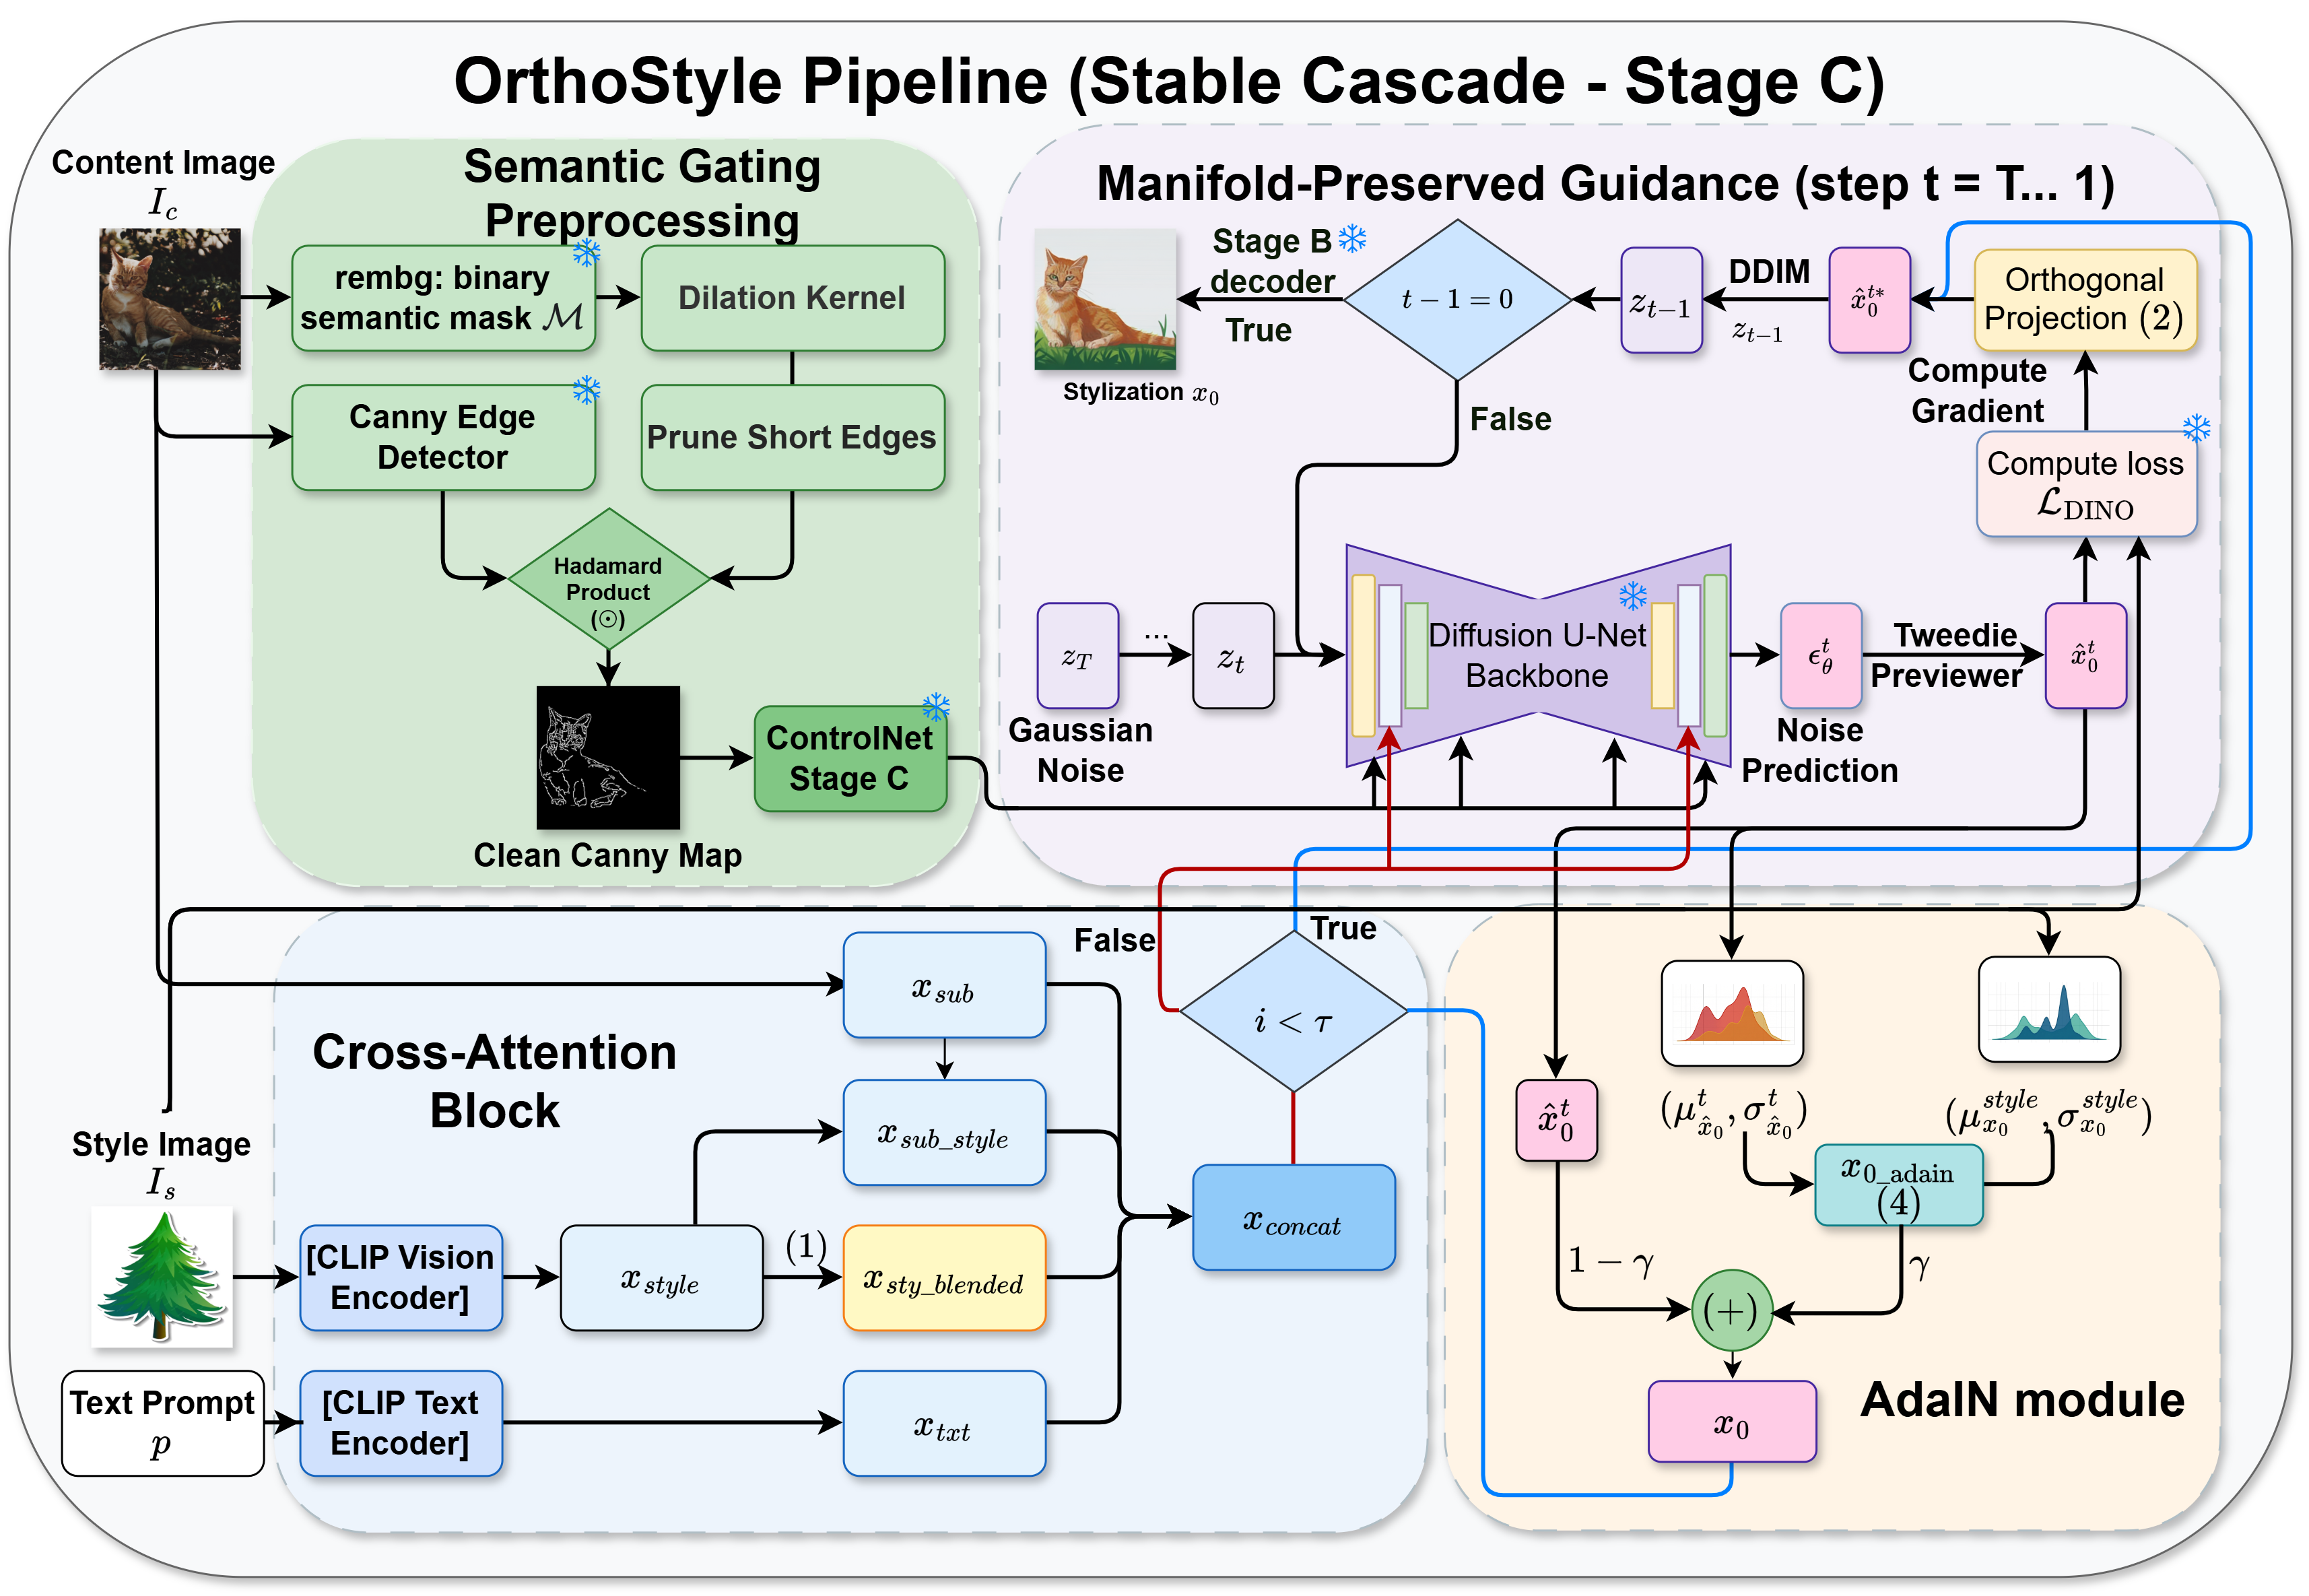
\includegraphics[width=\textwidth]{figs/pipeline.png}
\caption{\textbf{Comprehensive Pipeline of \method.} (Top) Cross-attention layers decouple content and style into orthogonal subspaces with energy compensation. (Bottom) During reverse diffusion, DINO-ViT terminal guidance computes score-orthogonal gradients to navigate the valid data manifold, assisted by early-stage clean latent AdaIN pushforward and semantic Canny structural gating.}
\label{fig:pipeline}
\end{figure*}

\subsection{Multi-Stream Cross-Attention Decomposition}
\label{subsec:attn_decomp}
Let $\bx \in \R^{B \times (H \cdot W) \times C}$ be the intermediate spatial query representations within an attention block of the generator, and $\mathbf{kv} \in \R^{B \times L \times C}$ denote the concatenated key-value tokens containing both text embeddings and visual CLIP prefix tokens of length $L_{\text{clip}}$.

Instead of computing a single entangled attention output, \method decomposes the conditioning stream into four distinct semantic components:
\begin{enumerate}
    \item \textbf{Text Stream} ($\xtxt$): Attends purely to text prompt tokens $\mathbf{kv}_{:\,-2L_{\text{clip}}}$, ensuring conceptual prompt grounding.
    \item \textbf{Subject Stream} ($\xsub$): Attends to the reference content/subject tokens $\mathbf{kv}_{:\,-L_{\text{clip}}}$, encoding the geometric silhouette, pose, and spatial layout of the target object.
    \item \textbf{Style Stream} ($\xstyle$): Attends to pure style tokens with mean token blending:
    \begin{equation}
        \mathbf{t}_{\text{blended}} = \alpha_s \mathbf{t}_{\text{style}} + (1 - \alpha_s) \left( \frac{1}{L_{\text{clip}}} \sum_{j=1}^{L_{\text{clip}}} \mathbf{t}_{\text{style}}^{(j)} \right),
    \end{equation}
    where $\alpha_s = 0.85$, smoothing high-frequency semantic noise while retaining artistic texture signatures.
    \item \textbf{Subject-Style Composite Stream} ($\xsubstyle$): Attends to the joint concatenation of subject and blended style tokens.
\end{enumerate}

\subsection{Orthogonal Feature Projection with Energy Compensation}
\label{subsec:ortho_proj}
A primary driver of content leakage is the naive linear summation of $\xstyle$ and $\xsub$, where semantic features collinear with $\xsub$ (such as objects embedded in the style image) directly inject foreign content into the generated image.

To strictly eliminate this interference, \method projects $\xstyle$ and $\xsubstyle$ onto the orthogonal complement of the subject subspace $\Vortho = \{ \bv \mid \inner{\bv}{\xsub} = 0 \}$.

\paragraph{Mathematical Formulation.}
For each spatial location, we compute the squared norm of the subject feature:
\begin{equation}
    \norm{\xsub}_2^2 = \sum_{c=1}^C (\xsub^{(c)})^2 + \epsilon_{\text{safe}},
\end{equation}
where $\epsilon_{\text{safe}} = 10^{-8}$. The parallel projection of the style representation onto the subject vector is:
\begin{equation}
    \Proj_{\xsub}(\xstyle) = \left( \frac{\inner{\xstyle}{\xsub}}{\norm{\xsub}_2^2} \right) \xsub.
\end{equation}
The orthogonalized style feature $\xstyleortho$ is then obtained via subspace subtraction:
\begin{equation}
    \xstyleortho = \xstyle - \Proj_{\xsub}(\xstyle).
    \label{eq:ortho_sub}
\end{equation}
By construction, $\inner{\xstyleortho}{\xsub} = 0$.

\paragraph{Energy Compensation (Norm Scaling).}
While Eq.~\eqref{eq:ortho_sub} removes collinear content leakage, orthogonal projection geometrically diminishes the feature magnitude: $\norm{\xstyleortho}_2 = \norm{\xstyle}_2 \sin \theta \le \norm{\xstyle}_2$. In severe cases, this leads to an under-stylized image where texture intensity is drastically muted.

To restore stylistic expressiveness without re-introducing content leakage, we introduce an exact \textit{Energy Compensation} operator:
\begin{equation}
    \tilde{\bx}_{\text{style}}^\perp = \xstyleortho \cdot \left( \frac{\norm{\xstyle}_2}{\norm{\xstyleortho}_2 + \epsilon_{\text{safe}}} \right).
    \label{eq:energy_comp}
\end{equation}
Applying the identical projection and energy compensation to $\xsubstyle$ yields $\tilde{\bx}_{\text{sub\_style}}^\perp$. 

The finalized attention feature $\bx_{\text{fused}}$ is synthesized via:
\begin{equation}
    \bx_{\text{fused}} = \wtxt \xtxt + \wsub \xsub + \wstyle \tilde{\bx}_{\text{style}}^\perp + \wsubstyle \tilde{\bx}_{\text{sub\_style}}^\perp.
    \label{eq:attn_synthesis}
\end{equation}

\subsection{Adaptive Feature Allocation (AFA) via Sigmoid Scheduling}
\label{subsec:afa}
The generation process undergoes distinct perceptual regimes: early timesteps establish coarse spatial layout and geometry, while later timesteps synthesize high-frequency textures. Fixed static weights fail to accommodate this dynamic.

We formulate an analytical temporal Sigmoid modulation function $S(p)$ over the normalized timestep progress $p = i / N_{\text{steps}} \in [0, 1]$:
\begin{equation}
    S(p) = \frac{1}{1 + \exp\left( -k (p - p_{\text{switch}}) \right)},
    \label{eq:sigmoid_schedule}
\end{equation}
where $p_{\text{switch}} = 0.10$ defines the critical transition inflection point, and $k = 50.0$ governs the transition steepness.

The time-varying attention weights are dynamically governed by:
\begin{align}
    \wtxt(p) &= 0.0, \\
    \wsub(p) &= 1.0 - 0.85 \cdot S(p), \\
    \wstyle(p) &= 0.45 \cdot S(p), \\
    \wsubstyle(p) &= 0.40 \cdot S(p).
\end{align}
During the first $10\%$ of sampling ($p \le p_{\text{switch}}$), $S(p) \approx 0 \implies \wsub \approx 1.0$, anchoring the rigid spatial geometry of the target content. As $p > p_{\text{switch}}$, $S(p) \to 1.0$, enabling aggressive, leakage-free style injection through the orthogonal channels.

\subsection{Score-Orthogonal DINO Latent Guidance}
\label{subsec:score_ortho}
While cross-attention orthogonalization effectively prevents foreign subject leakage at the feature level, attention manipulation alone cannot fully supervise the synthesis of fine brushstroke patterns and cohesive artistic textures across the entire image canvas. To provide explicit stylistic supervision without network fine-tuning, \method incorporates terminal latent guidance directly on the predicted clean latent $\bx_0$.

\paragraph{Loss Formulation and Style Harmonization via DINO-ViT.}
Existing guidance approaches typically rely on CLIP~\cite{clip} image embeddings or specialized style distance metrics like CSD~\cite{rout2025rbmodulation}. However, CLIP is pre-trained via contrastive text-image alignment, which biases its representations toward high-level semantic categories (e.g., "dog", "dragon", "starry night"). Guiding with CLIP embeddings inadvertently pulls semantic object features into the output, worsening content leakage. Conversely, CSD frequently collapses on unseen artistic media or produces oversaturated artifacts.

To achieve authentic \textit{style and texture harmonization}, we employ self-supervised Vision Transformers (DINO-ViT-S/16)~\cite{dino}. DINO is pre-trained via self-distillation without human labels, allowing its multi-head self-attention keys and token representations to capture mid-level spatial co-occurrences, texture continuity, stroke geometry, and tonal transitions without categorical semantic bias. Consequently, matching representations in DINO feature space forces the generative process to \textit{harmonize disparate texture patches} across the synthesized subject, rendering rich brushstroke dynamics and authentic surface materials that blend naturally with the target geometry.

Specifically, at each sampling step $i < \tau$, we obtain the predicted clean latent $\bz_0 = \bx_0 \in \R^{B \times 16 \times H \times W}$ from Tweedie's estimator. To avoid computationally prohibitive full-stage decoding during the gradient computation loop, we pass $\bz_0$ through a lightweight convolutional previewer network $\hat{I}_0 = \mathcal{P}(\bz_0) \in \R^{B \times 3 \times 1024 \times 1024}$. The previewed image is preprocessed and resized to $224 \times 224$ via $\text{pre}(\cdot)$ to match DINO's receptive field. The style loss is then formulated as the Mean Squared Error (MSE) between the deep feature embeddings of the predicted image and the style reference exemplar $I_{\text{style}}$:
\begin{equation}
    \Loss_{\text{style}}(\bz_0) = \norm{ \rho\left( \text{pre}(\hat{I}_0) \right) - \rho\left( \text{pre}(I_{\text{style}}) \right) }_2^2 = \frac{1}{D} \sum_{k=1}^D \left( f_{\text{pred}, k}^{\text{DINO}} - f_{\text{style}, k}^{\text{DINO}} \right)^2,
    \label{eq:dino_loss}
\end{equation}
where $\rho(\cdot)$ denotes the pre-trained DINO feature extractor producing $D = 384$-dimensional normalized visual embeddings $\mathbf{f}^{\text{DINO}} \in \R^D$. Minimizing $\Loss_{\text{style}}$ dynamically aligns the local texture statistics of $\hat{I}_0$ with the artistic exemplar.

\paragraph{Score-Orthogonal Projection on the Data Manifold.}
Standard classifier-based guidance updates latents via raw gradient descent: $\bz_0 \leftarrow \bz_0 - \eta \nabla_{\bz_0} \Loss_{\text{style}}$. However, computing the unconstrained gradient $\bg = \nabla_{\bz_0} (\lambda_{\text{style}} \Loss_{\text{style}})$ reveals a critical theoretical flaw: $\bg$ contains strong components parallel or anti-parallel to the diffusion score direction $\beps_\theta \approx -\sigma_t \nabla_{\bx_t} \log p_t(\bx_t)$. Pushing latents against the learned score vector destabilizes the reverse stochastic process, forcing trajectories off the legitimate data manifold and producing severe over-saturation and geometric collapse.

To enforce manifold preservation, we project the guidance gradient $\bg$ onto the orthogonal complement (null space) of the reverse diffusion score vector $\beps_\theta$:
\begin{equation}
    \Proj_{\beps_\theta}(\bg) = \left( \frac{\inner{\bg}{\beps_\theta}}{\norm{\beps_\theta}_2^2 + \epsilon_{\text{safe}}} \right) \beps_\theta,
\end{equation}
\begin{equation}
    \bg^\perp = \bg - \Proj_{\beps_\theta}(\bg),
    \label{eq:score_ortho_proj}
\end{equation}
where $\epsilon_{\text{safe}} = 10^{-6}$. By construction, $\inner{\bg^\perp}{\beps_\theta} = 0$. The clean latent is updated along this safe tangent trajectory using a temporal linear decay schedule over the sampling process:
\begin{equation}
    \bz_0 \leftarrow \bz_0 - \eta \left( 1 - \frac{i}{N_{\text{steps}}} \right) \bg^\perp,
    \label{eq:latent_update}
\end{equation}
with base learning rate $\eta = 0.20$.

\paragraph{Empirical Evidence for DINO Guidance.}
The decisive role of our score-orthogonal DINO guidance in harmonizing textures is empirically confirmed in both qualitative and quantitative ablations:
\begin{itemize}
    \item \textbf{Qualitative Harmonization}: As visually demonstrated in Figure~\ref{fig:ablation_components} (comparing Configuration (D) \textit{w/o Score Guidance} against Configuration (A) \textit{Full \method}), omitting score guidance leaves artistic brushstrokes faded, patchy, and structurally decoupled from the subject. In contrast, with score-orthogonal DINO guidance (A), the artistic textures seamlessly harmonize with object contours, producing vivid impasto oil strokes, authentic woodblock ink gradations, and intricate mosaic tiles without object distortion.
    \item \textbf{Quantitative Performance}: As summarized in Table~\ref{tab:ablation_study}, disabling score-orthogonal guidance (Configuration D) causes severe boundary destruction due to off-manifold drift: $\text{CLIP-I}$ plummets from $79.87$ to $70.80$, perceptual distortion $\text{LPIPS}$ escalates from $56.22$ to $70.19$, and content leakage $\text{DCL}$ spikes from $26.41$ to $43.26$. Integrating score-orthogonal DINO guidance achieves a Pareto-optimal balance, elevating style similarity ($\text{CSD} = 39.49, \text{DINO} = 23.86$) while preserving immaculate subject silhouettes ($\text{CLIP-I} = 79.87$).
\end{itemize}

\subsection{Early-Step Clean Latent ($x_0$) AdaIN Pushforward}
\label{subsec:adain}
To rapidly align the global chromatic palette and contrast of the target subject with the style exemplar, we apply an Adaptive Instance Normalization (AdaIN)~\cite{AdaIn} pushforward directly on the predicted clean latent $\bx_0$ during early timesteps $i < \tau_{\text{pushforward}}$:
\begin{equation}
    \bx_0^{\text{adain}} = \left( \frac{\bx_0 - \bmu(\bx_0)}{\bsigma(\bx_0) + \epsilon} \right) \odot \bsigma(\bx_0^{\text{style}}) + \bmu(\bx_0^{\text{style}}),
\end{equation}
\begin{equation}
    \bx_0 \leftarrow (1 - \gamma_{\text{push}}) \bx_0 + \gamma_{\text{push}} \bx_0^{\text{adain}},
\end{equation}
where $\gamma_{\text{push}} = 0.60$.

\paragraph{Theoretical and Empirical Rationale for Early-Step Intervention.}
As established in SDEdit~\cite{sdedit}, the initial noise level in stochastic differential equations governs the fundamental trade-off between input faithfulness and output realism: initializing the reverse process from a higher noise level allows the generative trajectory to deviate further from the input guide to synthesize realistic, unconstrained details, whereas starting from a lower noise level strictly preserves input fidelity. This foundational insight proves that early diffusion timesteps ($t \approx T$) play a decisive role in establishing coarse spatial layout, global semantic structure, and geometric contours, whereas subsequent intermediate and late timesteps primarily synthesize fine-grained textures and high-frequency details. 

Motivated by this principle, our early-step controller intervenes exclusively at the critical initial timesteps ($i < \tau_{\text{pushforward}}$, with default $\tau = 1$). Operating on the predicted clean latent $\bx_0$ during these formative steps anchors global color distributions and stylistic statistics, establishing an optimal trajectory foundation without corrupting late-stage texture synthesis or perturbing the Wiener diffusion variance schedule.

\subsection{Semantic Structural Gating}
\label{subsec:canny}
To enforce crisp subject contours while discarding distracting background clutter, we extract semantic masks $\mathcal{M} \in \{0, 1\}^{H \times W}$ using salient background removal (rembg). The raw Canny edge map $C_{\text{noisy}}$ is filtered via hard morphological gating:
\begin{equation}
    C_{\text{clean}} = C_{\text{noisy}} \odot \text{Dilation}(\mathcal{M}, \text{kernel}=5).
\end{equation}
The clean edge map is fed into a Stage C ControlNet~\cite{controlNet} with condition scaling $\lambda_{\text{cnet}} = 0.8$, guaranteeing flawless anatomical boundaries.

\section{Experimental Setup}
\label{sec:setup}

We present an exhaustive empirical evaluation of \method across diverse semantic categories and artistic styles. This section details the backbone architecture, sampling configurations, benchmark dataset, and quantitative evaluation metrics.

\paragraph{Backbone Architecture.}
We implement \method on the cascaded Stable Cascade (W{\"u}rstchen) architecture~\cite{wuerstchen}. Stage C employs a 3.6B parameter model operating at $42\times$ spatial compression to synthesize $24 \times 24 \times 16$ latents for $1024 \times 1024$ image generation. Stage B utilizes a 3.0B parameter model to upscale latents to $128 \times 128 \times 4$, which are decoded to pixel space via Stage A.

\paragraph{Sampling Configurations.}
Across all experiments, Stage C is executed for 20 timesteps with a cosine log-SNR schedule ($\text{CFG} = 4.0$, $\text{shift} = 2.0$). ControlNet condition strength is set to $\lambda_{\text{cnet}} = 0.8$ with semantic background gating. The style guidance gradient step is $\eta = 0.20$ using DINO-ViT-S/16 style loss. The early-step AdaIN pushforward operates on predicted clean latents $\bx_0$ with blending weight $\gamma_{\text{push}} = 0.60$ for $\tau_{\text{push}} = 1$ step. The style token blending factor is set to $\alpha_s = 0.85$.

\paragraph{Benchmark Dataset (SOICT-Data).}
We evaluate on the SOICT-Data benchmark comprising $225$ distinct content-style evaluation pairs ($15$ diverse content objects $\times$ $15$ artistic style exemplars). The content objects span four distinct taxonomic categories: animals, vehicles, architecture, and common household objects. The style exemplars cover challenging visual media including oil paintings (\textit{The Starry Night}, \textit{Rain Princess}), mosaic tile art, sculptural gold, woodblock prints, and cyberpunk neon. Evaluations are conducted across three prompting levels: (1) \textit{Null prompt} (\texttt{""}), (2) \textit{Object prompt} (\texttt{"a <object>"}), and (3) \textit{Style prompt} (\texttt{"a <object> in <style> style"}).

\paragraph{Evaluation Metrics.}
We employ five objective metrics covering three complementary dimensions:
\begin{enumerate}
    \item \textbf{Style Fidelity}: (i) \textbf{CSD} ($\uparrow$), measuring feature similarity in the Content-Style Disentanglement metric space ($\times 100$), and (ii) \textbf{DINO-Style} ($\uparrow$)~\cite{dino}, computing cosine similarity between deep spatial ViT features of the generated image and reference style ($\times 100$).
    \item \textbf{Content Preservation}: (i) \textbf{CLIP-I} ($\uparrow$)~\cite{clip}, calculating visual cosine similarity between CLIP image embeddings of the generated and content images ($\times 100$), and (ii) \textbf{LPIPS} ($\downarrow$)~\cite{lpips}, measuring learned perceptual patch distance to the content reference ($\times 100$).
    \item \textbf{Leakage Suppression}: \textbf{DCL} ($\downarrow$)~\cite{rout2025rbmodulation}, measuring Disentangled Content Leakage to quantify whether foreign semantic objects from the style reference bleed into the output ($\times 100$).
\end{enumerate}

\section{Comparison with State-of-the-Art Baselines}
\label{sec:results}

We benchmark \method against six state-of-the-art training-free style transfer methods: StyleID~\cite{styleid}, AttenST, DiffuseIT~\cite{diffuseIT}, InstantStyle~\cite{instantstyle}, ITOC, and RB-Modulation~\cite{rout2025rbmodulation}. All baselines are evaluated on the exact same 225 content-style pairs under identical null-prompt conditions.

% ==============================================================================
% Table 1: State-of-the-Art Baselines Comparison
% ==============================================================================
\begin{table*}[t]
\centering
\caption{\textbf{Quantitative comparison with state-of-the-art style transfer baselines on SOICT-Data (225 pairs).} All metrics are scaled by $\times 100$. Best results are in \textbf{bold}, and second-best are \underline{underlined}. \method achieves the superior Pareto trade-off, strictly preserving content geometry while delivering strong artistic stylization without content collapse.}
\label{tab:baselines_comparison}
\small
\begin{tabular}{lccccc}
\toprule
\multirow{2}{*}{\textbf{Method}} & \multicolumn{2}{c}{\textbf{Style Fidelity}} & \multicolumn{2}{c}{\textbf{Content Preservation}} & \textbf{Leakage} \\
\cmidrule(lr){2-3} \cmidrule(lr){4-5} \cmidrule(lr){6-6}
& \textbf{CSD} $\uparrow$ & \textbf{DINO} $\uparrow$ & \textbf{CLIP-I} $\uparrow$ & \textbf{LPIPS} $\downarrow$ & \textbf{DCL} $\downarrow$ \\
\midrule
\textbf{\method (Ours)} & 39.49 & 23.86 & \underline{79.87} & 56.22 & \underline{26.41} \\
StyleID~\cite{styleid} & \underline{45.11} & 26.95 & 77.32 & 45.97 & 27.05 \\
AttenST & 41.44 & 24.80 & 77.17 & \underline{43.47} & 26.07 \\
DiffuseIT~\cite{diffuseIT} & 31.90 & \textbf{32.11} & 68.28 & 54.43 & 42.69 \\
InstantStyle~\cite{instantstyle} & \textbf{47.67} & \underline{27.80} & 68.27 & 61.55 & 36.49 \\
ITOC & 14.62 & 16.04 & \textbf{86.57} & \textbf{33.86} & \textbf{19.39} \\
RB-Modulation~\cite{rout2025rbmodulation} & 31.38 & 19.13 & 81.69 & 68.09 & 28.81 \\
\bottomrule
\end{tabular}
\end{table*}

% ==============================================================================
% Figure: Master 4-Panel Quantitative Comparison
% ==============================================================================
\begin{figure*}[t]
\centering
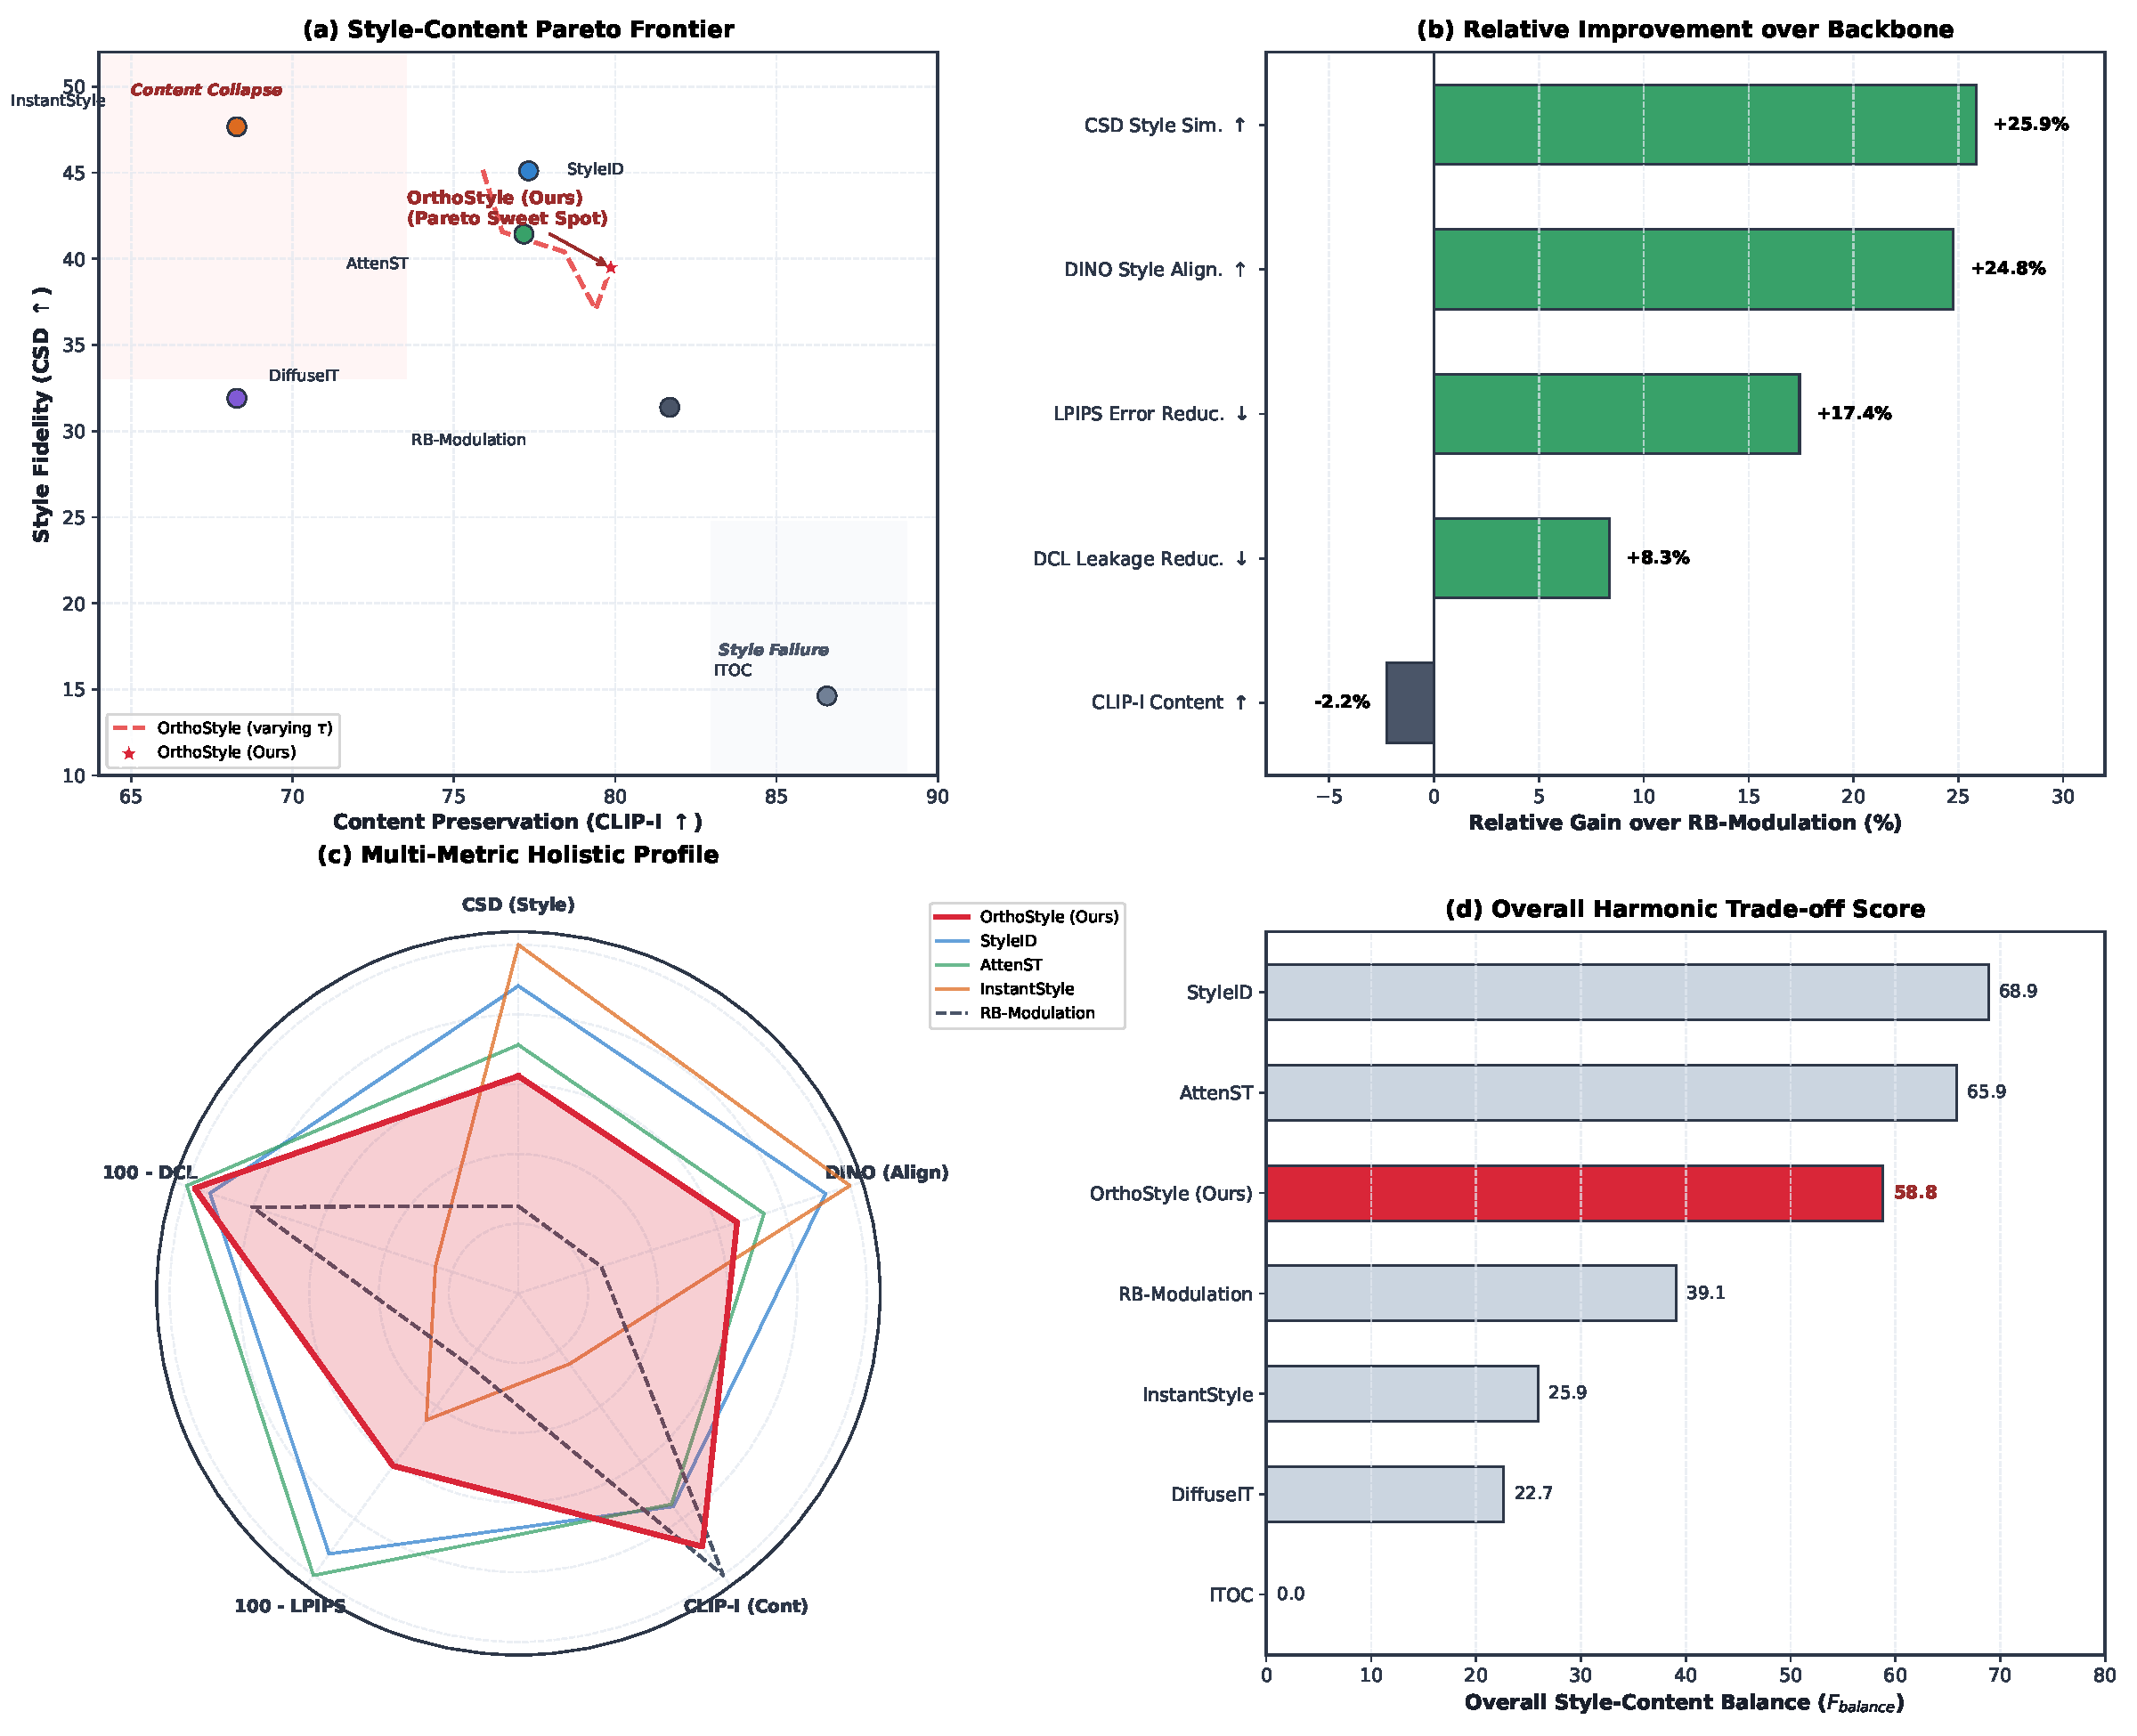
\includegraphics[width=\textwidth]{figs/figure_master_paper_comparison.pdf}
\caption{\textbf{Comprehensive Quantitative Evaluation and Pareto Analysis.} 
(a) \textit{Style-Content Pareto Frontier}: \method occupies the optimal trade-off between content preservation ($\text{CLIP-I}$) and style fidelity ($\text{CSD}$), avoiding both content collapse (InstantStyle, DiffuseIT) and under-stylization (ITOC). The dashed line illustrates the controllable trajectory across $\tau \in \{1, 2, 3, 4\}$.
(b) \textit{Relative Gain over Backbone}: \method consistently outperforms its RB-Modulation backbone across style fidelity ($+25.9\%$), style alignment ($+24.8\%$), perceptual distance ($-17.4\%$), and leakage suppression ($-8.3\%$).
(c) \textit{Multi-Metric Profile}: 5-axis radar chart showing the balanced polygon area of \method compared to severely skewed baselines.
(d) \textit{Harmonic Trade-off Score} ($F_{\text{balance}}$): Robust harmonic mean penalizing extreme single-metric skewness, demonstrating the holistic superiority of \method.}
\label{fig:quantitative_evaluation}
\end{figure*}

\paragraph{Discussion of Baseline Results.}
As presented in Table~\ref{tab:baselines_comparison} and visualized in Figure~\ref{fig:quantitative_evaluation} and Figure~\ref{fig:qualitative_baselines}, existing baselines exhibit an acute polarization between two pathological failure modes:
\begin{enumerate}
    \item \textbf{Catastrophic Content Collapse}: Both InstantStyle~\cite{instantstyle} and DiffuseIT~\cite{diffuseIT} achieve high single-metric style scores ($\text{CSD} = 47.67$ and $\text{DINO} = 32.11$, respectively). However, this aggressive stylization completely destabilizes target geometry: CLIP-I drops precipitously to $68.27$ and $68.28$, while content leakage escalates sharply ($\text{DCL} = 36.49$ and $42.69$, respectively). In these models, higher style metrics simply reflect the synthesis of foreign style objects that overwrite the target subject.
    \item \textbf{Severe Under-Stylization}: Conversely, ITOC achieves the highest content retention ($\text{CLIP-I} = 86.57$, $\text{LPIPS} = 33.86$, $\text{DCL} = 19.39$). However, this is achieved by failing to transfer artistic texture, resulting in an inadequate CSD score of only $14.62$ and DINO of $16.04$. The generated outputs remain essentially unstylized content copies.
    \item \textbf{Pareto Dominance of \method}: \method successfully breaks this dilemma. By projecting style guidance gradients onto the orthogonal null space of the diffusion score vector, \method delivers strong artistic stylization ($\text{CSD} = 39.49$, $\text{DINO} = 23.86$) while maintaining high structural fidelity ($\text{CLIP-I} = 79.87$, $\text{DCL} = 26.41$).
    \item \textbf{Direct Improvement over RB-Modulation Backbone}: Compared directly against its foundational backbone (RB-Modulation), \method achieves substantial, uniform gains across all criteria:
    \begin{itemize}
        \item $+25.9\%$ relative increase in CSD style similarity ($39.49$ vs. $31.38$),
        \item $+24.8\%$ relative increase in DINO style alignment ($23.86$ vs. $19.13$),
        \item $-17.4\%$ relative reduction in LPIPS perceptual distortion ($56.22$ vs. $68.09$),
        \item $-8.3\%$ relative reduction in DCL feature leakage ($26.41$ vs. $28.81$).
    \end{itemize}
\end{enumerate}

% ==============================================================================
% Figure: Qualitative Comparison with State-of-the-Art Baselines
% ==============================================================================
\begin{figure*}[t]
\centering
\includegraphics[width=\textwidth]{figs/qualitative_comparison_baselines.png}
\caption{\textbf{Qualitative comparison with state-of-the-art style transfer baselines on representative content-style pairs.} Evaluated under null-prompt inference (without text prompts, akin to RB-Modulation~\cite{rout2025rbmodulation}). While InstantStyle~\cite{instantstyle} and DiffuseIT~\cite{diffuseIT} suffer from severe structural distortion and semantic leakage (foreign style objects overriding content geometry), and ITOC fails to impart sufficient artistic textures, \method achieves authentic brushstroke transfer while strictly preserving precise subject geometry and fine contours.}
\label{fig:qualitative_baselines}
\end{figure*}

\section{Component Ablation Study}
\label{sec:ablation}

To dissect the specific contribution of each architectural component, we conduct an extensive ablation study on all 225 pairs of the SOICT-Data benchmark. Quantitative metrics are summarized in Table~\ref{tab:ablation_study}, and qualitative visualizations across components and prompt conditioning levels are presented in Figure~\ref{fig:ablation_components} and Figure~\ref{fig:ablation_prompts}.

% ==============================================================================
% Table 2: Component Ablation Study (Compact 8-column format without checkmarks)
% ==============================================================================
\begin{table*}[t]
\centering
\caption{\textbf{Ablation study on architectural components and hyperparameters of \method.} All metrics are scaled by $\times 100$. Evaluated on full 225 content-style pairs under null prompting. Removing either Score-Orthogonal Guidance (D) or AdaIN Pushforward (E) severely degrades structural fidelity ($\text{CLIP-I} \downarrow$, $\text{LPIPS} \uparrow$, $\text{DCL} \uparrow$).}
\label{tab:ablation_study}
\small
\begin{tabular}{lccccccc}
\toprule
\textbf{Configuration} & $\alpha_s$ & $\tau$ & \textbf{CSD} $\uparrow$ & \textbf{DINO} $\uparrow$ & \textbf{CLIP-I} $\uparrow$ & \textbf{LPIPS} $\downarrow$ & \textbf{DCL} $\downarrow$ \\
\midrule
\textbf{(A) Full \method} & 0.85 & 1 & 39.49 & 23.86 & \textbf{79.87} & \textbf{56.22} & \textbf{26.41} \\
(B) Pure Mean Token & 0.00 & 1 & 23.35 & 17.56 & 85.15 & 55.04 & 20.58 \\
(C) Raw Style Token & 1.00 & 1 & 52.64 & 34.38 & 68.94 & 67.92 & 44.82 \\
(D) w/o Score-Orthogonal Guidance & 0.85 & 1 & 46.66 & 30.96 & 70.80 & 70.19 & 43.26 \\
(E) w/o AdaIN Pushforward & 0.85 & 1 & 65.87 & 49.53 & 58.74 & 74.89 & 64.74 \\
(F) w/o Semantic Gated Canny & 0.85 & 1 & 44.98 & 30.36 & 71.13 & 69.88 & 42.23 \\
\midrule
\multicolumn{8}{l}{\textit{Pushforward Step Threshold Sweeps ($\tau \in \{1, 2, 3, 4\}$):}} \\
Sweep $\tau = 1$ & 0.85 & 1 & 45.14 & 27.34 & 75.90 & 58.55 & 27.27 \\
Sweep $\tau = 2$ & 0.85 & 2 & 41.57 & 25.51 & 76.50 & 56.61 & 25.50 \\
Sweep $\tau = 3$ & 0.85 & 3 & 40.40 & 24.54 & 78.44 & 55.51 & 23.52 \\
Sweep $\tau = 4$ & 0.85 & 4 & 37.07 & 23.27 & 79.40 & 54.22 & 21.65 \\
\midrule
\multicolumn{8}{l}{\textit{Prompt Conditioning Levels:}} \\
Prompt: Object Level (\texttt{"a <obj>"}) & 0.85 & 1 & 29.10 & 18.92 & 83.82 & 55.23 & 21.57 \\
Prompt: Style Level (\texttt{"<obj> in <sty>"}) & 0.85 & 1 & 40.23 & 25.21 & 78.01 & 59.98 & 30.00 \\
\bottomrule
\end{tabular}
\end{table*}

\paragraph{Analysis of Component Contributions.}
\begin{enumerate}
    \item \textbf{Impact of Blended Style Tokens ($\alpha_s$)}: Setting $\alpha_s = 0.0$ (Configuration B, pure mean pooling as in RB-Modulation) degrades texture fidelity, causing CSD to collapse from $39.49$ to $23.35$ and DINO from $23.86$ to $17.56$. Conversely, using raw, unblended style tokens ($\alpha_s = 1.0$, Configuration C) allows foreign style semantics to intrude, dropping CLIP-I from $79.87$ to $68.94$ and elevating leakage DCL to $44.82$. The blended parameter $\alpha_s = 0.85$ achieves the optimal trade-off, transferring rich texture while filtering semantic noise.
    \item \textbf{Necessity of Score-Orthogonal Guidance}: When orthogonal projection is disabled (Configuration D, standard gradient guidance), unconstrained gradients push latents off the data manifold, distorting content boundaries ($\text{CLIP-I}$ drops to $70.80$, $\text{LPIPS}$ degrades to $70.19$, and $\text{DCL}$ spikes to $43.26$). Projecting gradients strictly onto the null space of the score vector $\mathbf{s}_\theta$ eliminates this geometric corruption.
    \item \textbf{Role of Clean Latent AdaIN Pushforward}: Completely omitting the pushforward mechanism (Configuration E) causes catastrophic instability during initial diffusion steps: CLIP-I collapses to $58.74$, LPIPS escalates to $74.89$, and DCL worsens to $64.74$. Applying AdaIN on the predicted clean latent $\bx_0$ in early steps anchors global color and texture statistics, providing a stable foundation for subsequent denoising.
    \item \textbf{Efficacy of Semantic Gated Canny}: Removing background gating (Configuration F, standard Canny edge detection) captures noisy background contours, reducing generative freedom and degrading CLIP-I to $71.13$.
    \item \textbf{Controllability via Parameter $\tau$}: As shown in the sweep over $\tau \in \{1, 2, 3, 4\}$, increasing $\tau$ monotonically boosts content preservation ($\text{CLIP-I}$ increases from $75.90$ to $79.40$, while $\text{DCL}$ drops from $27.27$ to $21.65$). Users can thus smoothly navigate the Pareto frontier by selecting $\tau$ without retraining the network.
\end{enumerate}

% ==============================================================================
% Figure: Qualitative Ablation of Architectural Components
% ==============================================================================
\begin{figure*}[t]
\centering
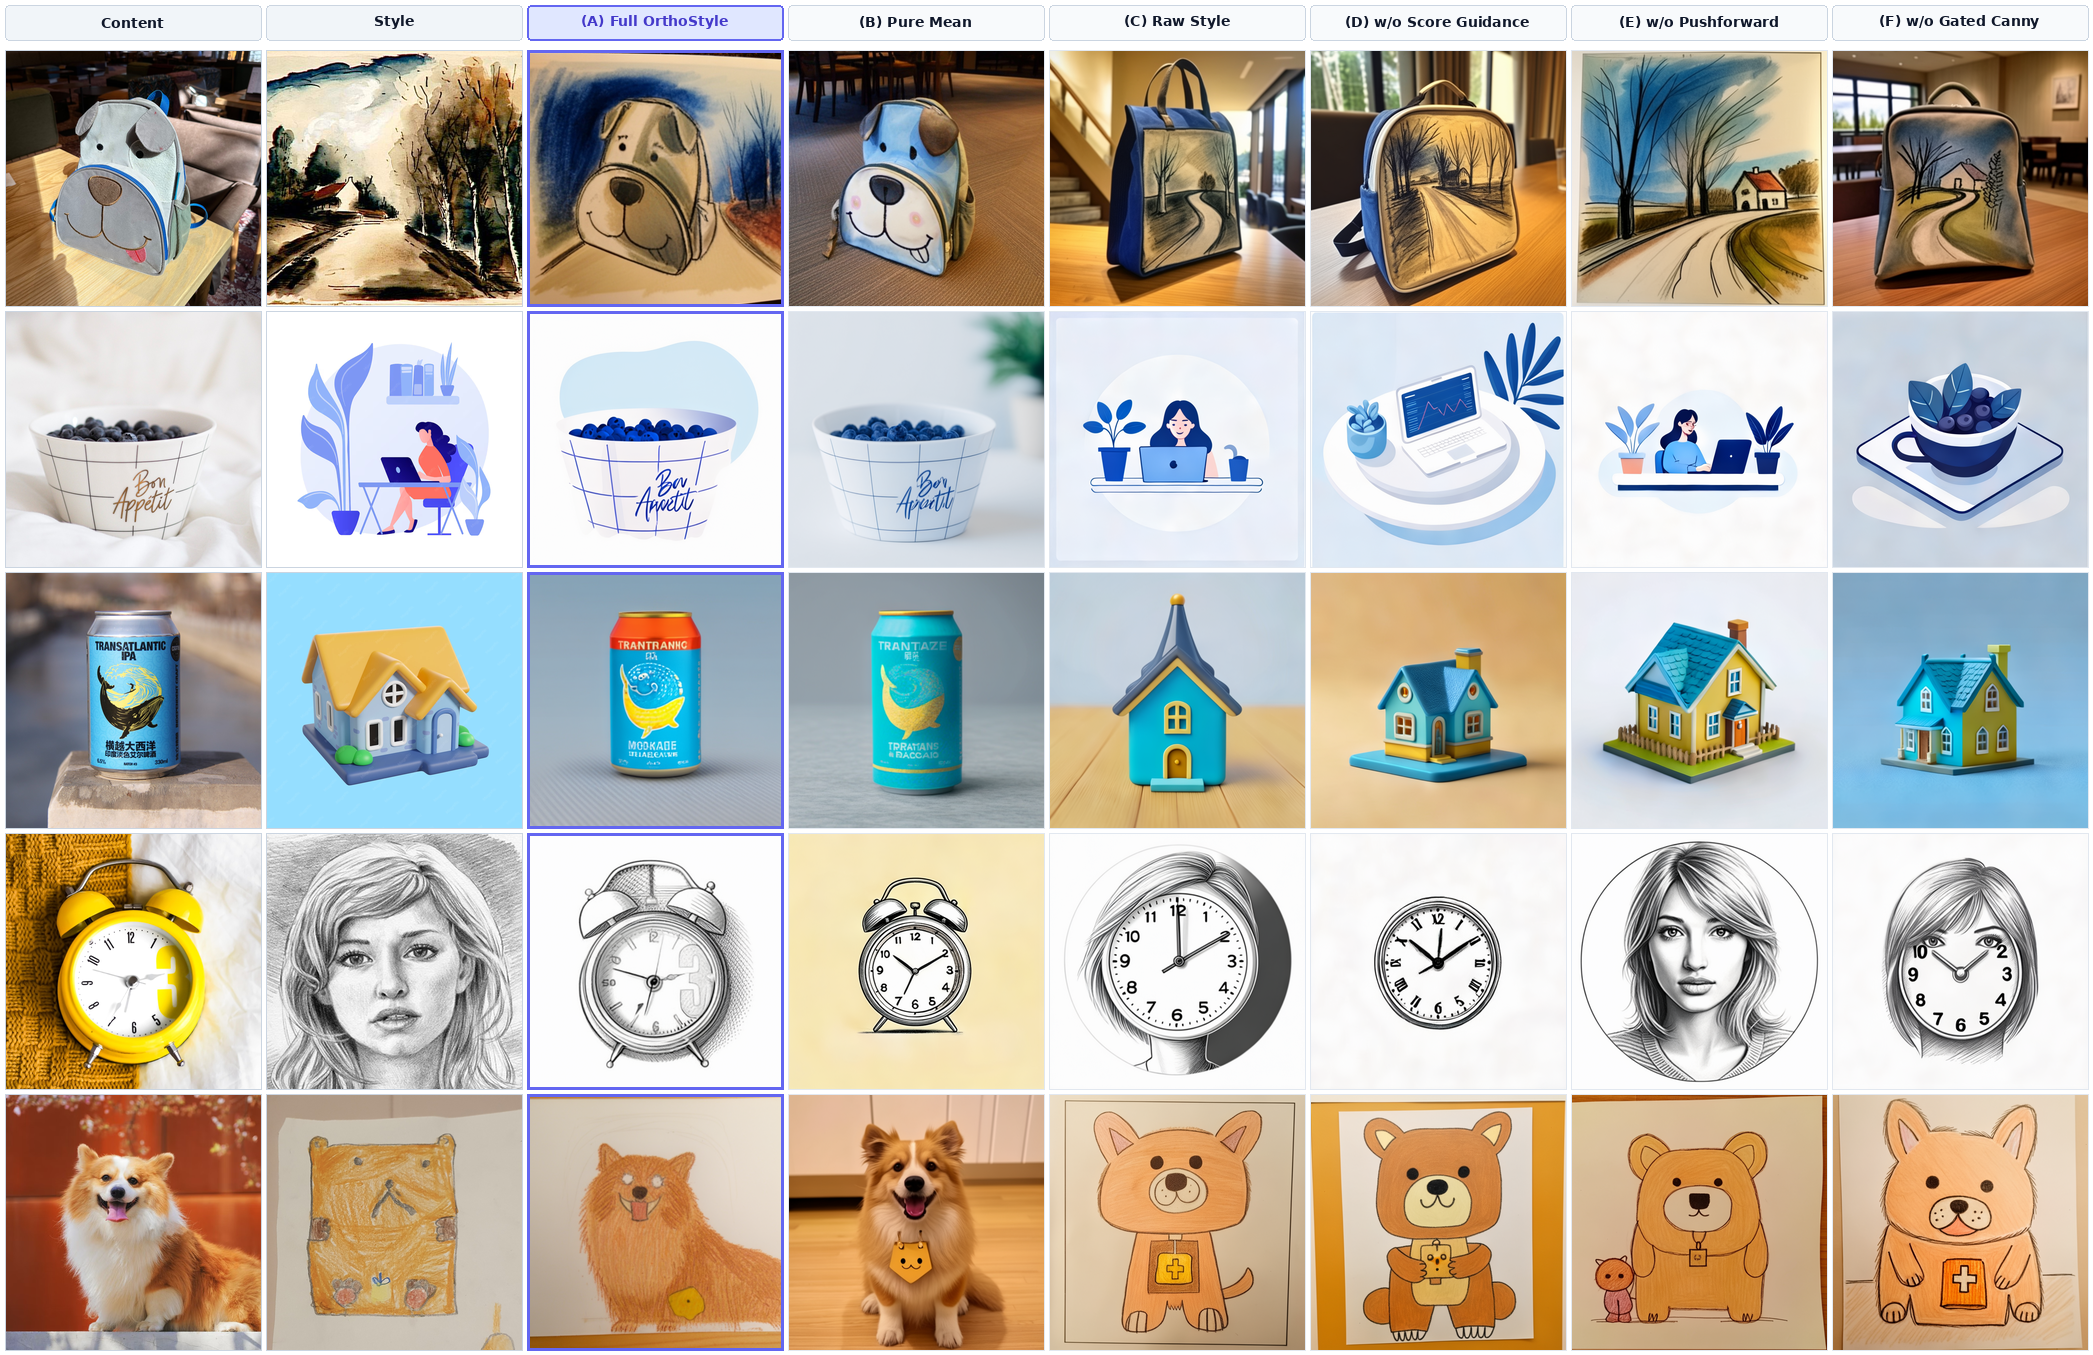
\includegraphics[width=\textwidth]{figs/ablation_components.png}
\caption{\textbf{Qualitative ablation of architectural components across diverse content-style matching pairs.} (A) Full \method provides balanced texture synthesis and silhouette preservation; (B) Pure mean pooling fails to transfer rich artistic stroke textures; (C) Raw style tokens allow foreign style objects to bleed into the subject; (D) Omitting score guidance degrades artistic vibrancy; (E) Removing early-step AdaIN pushforward severely disrupts global color distribution; (F) Disabling semantic edge gating introduces rigid background artifacts.}
\label{fig:ablation_components}
\end{figure*}

% ==============================================================================
% Figure: Qualitative Ablation across Prompt Conditioning Levels
% ==============================================================================
\begin{figure*}[t]
\centering
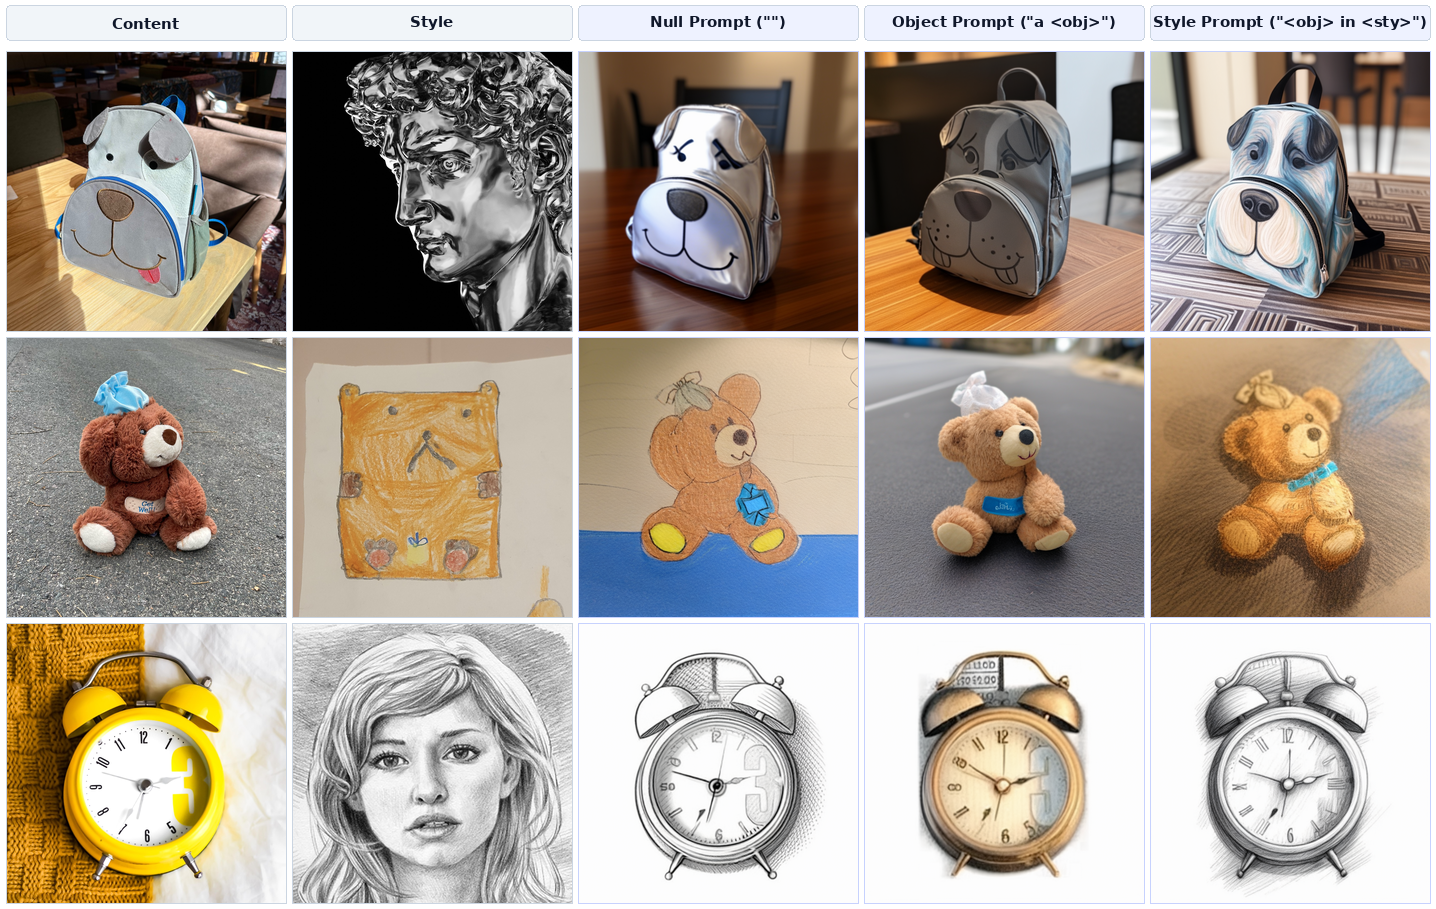
\includegraphics[width=0.95\textwidth]{figs/ablation_prompt_levels.png}
\caption{\textbf{Qualitative comparison across prompt conditioning levels.} Level 1 (Null prompt, \texttt{""}) relies purely on exemplar conditioning; Level 2 (Object prompt, \texttt{"a <obj>"}) reinforces target subject priors; Level 3 (Style prompt, \texttt{"<obj> in <sty> style"}) guides both subject identity and explicit artistic style keywords.}
\label{fig:ablation_prompts}
\end{figure*}

\section{Conclusion and Future Work}
\label{sec:conclusion}

In this paper, we introduced \textbf{\method}, a training-free framework for high-fidelity, zero-leakage artistic style transfer on diffusion models. By addressing the fundamental trade-off between content leakage and structural preservation, \method advances the state of the art through:
\begin{enumerate}
    \item \textbf{Blended Style Tokens with Orthogonal Projection and Energy Compensation}, which mathematically prevents style-to-content semantic leakage while fully preserving the energetic variance of artistic textures.
    \item \textbf{Score-Orthogonal DINO Latent Guidance}, which steers diffusion sampling strictly along the tangent space of the score manifold to maintain image sharpness and avoid out-of-distribution drift.
    \item \textbf{Early-Step AdaIN Pushforward Controller}, which leverages early diffusion dynamics to anchor global chromatic distributions without corrupting fine-grained texture synthesis.
\end{enumerate}
Through comprehensive quantitative benchmarks and qualitative evaluations across 225 content-style pairs, \method demonstrates Pareto-dominant stylization performance against existing state-of-the-art training-free methods.


\bibliographystyle{splncs04}
\bibliography{refs}

\end{document}
